\section{Research methodology}\label{research-methodology}

{[}Revision 3{]}

changelog

\begin{itemize}
\itemsep1pt\parskip0pt\parsep0pt
\item
  removed interpretative case studies as methodologies
\item
  removed instantiation of (March, 1995) framework
\item
  Added instantiation of (Havner, 2007) framework, a better fit for the
  type of work done
\item
  Added tables for field studies, prototypes and focus groups
\item
  added figures
\end{itemize}

The aims of this chapter are to present the research design, to describe
methods and tools adopted and how data have been analysed. Although not
all of these methods and results have been explicitly reported in the
papers, they have been important to understand the users, the domain and
the needs. The adopted methods weren't given a priori but rather they
emerged over time.

\subsection{Research overview}\label{research-overview}

The work in this thesis is based on design research {[}@Hevner:2010fy;
@March:1995gm{]}. Design science provides theoretical tools to study and
understand a specific domain and processes to build artefacts with the
aim at improving an environment {[}@simon1996sciences{]}. The work
unfolded by interweaving field studies to understand a specific setting
and turn opportunities observed into system requirements; with design
iterations to build technologies to address those opportunities. The
design artifacts produced were both useful for understanding the domain
and in adding new knowledge to the domain.

The design science approach meet the aim of this research work, which
lies not only in building an understanding of the crisis domain but also
in contributing with the design of technologies for better crisis
training (RQ1-RQ2). The focus of design science on rapid iterations
between the construction of artifacts and their evaluation
{[}@Hevner:2010gc{]} makes also a good strategy for the investigation of
RQ3.

Hevner {[}-@Havner2004; -@hevner2007three{]} describes design research
as a sequence of three tightly coupled cycles of activities (Figure X).
And each of the three cycles must be present and visible in a design
science research project {[}@Hevner:2010gc{]}.

\begin{figure}[htbp]
\centering
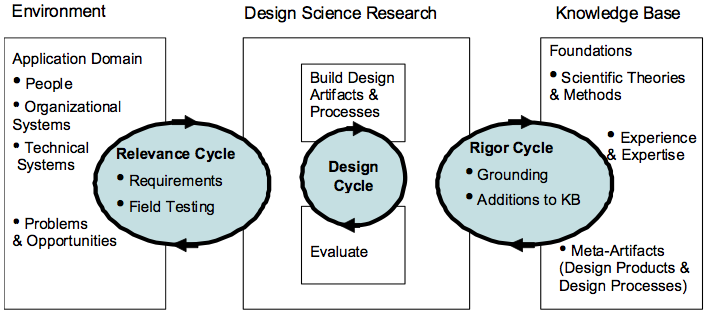
\includegraphics{imgs/design_cycles.png}
\caption{The design cycles, figure adapted from {[}@hevner2007three{]}}
\end{figure}

The \emph{relevance cycle} initiates the research by identifying
opportunities and problems for a specific domain and deriving
requirements for the design of technology to address those. Once the
requirements are implemented in design artefacts, acceptance criteria
for the summative evaluation are defined and artefacts are introduced
into the environment for field testing. Results from field evaluations
inform new cycle iterations until research goals are met. \textbf{This
stage involves designing running field studies with exploratory or
evaluation purposes}.

The \emph{rigor cycle} instantiates grounding theories and methods into
design activities, and it contributes into the knowledge base with new
constructs generated by research. The cycle provides past knowledge to
drive design work and to ensure it maintains an innovation approach able
to bring research contributions. At the same time, extensions or
generalisations of existing theories together with new constructs,
knowledge and methods generated by the design process are added to the
knowledge base. \textbf{This stage includes a continuous process of
keeping design work informed by relevant grounding theory and a
retrospective theoretical work of validating and extending these
theories}.

The \emph{design cycle} iterates between the production of an artifact,
its formative evaluation and it derives feedbacks to further refine the
design. The cycle is fed with requirements from the relevance cycle and
theories from the rigor cycle; it returns artefacts for field test to
the former and knowledge to the advances of theories to the latter. This
cycle is characterised by rapid iterations where small incremental
improvements in design artefacts are tested before an artefact is
released into the field or new knowledge is added to the rigor cycle.
\textbf{This stage involves the construction of prototypes and
successive lab tests}.

To support the cycles activities several research methods were adopted.
Observations, interviews and researchers' notes were the primary means
to collect data on the field. We used a mix of qualitative and
quantitative research methods to account for the unpredictability in an
in-situ study {[}@Rogers:2007gv{]}. Scenarios and personas drove the
design phase. Open source hardware and software tools were largely
adopted to turn mockups into working prototypes. Finally questionnaires
and interviews, interviews were used during prototypes evaluations.

The choice of these methods required the researchers to have large
access to people, knowledge and protocols of organisations working in
the crisis domain. This research strategy was facilitated by having
crisis response organisations member of the MIRROR consortium. Moreover,
throughout the duration of the work, discussions with members of MIRROR
during project meetings and workshops helped in shaping design choices
and partially influenced the work.

The following section details on what research activities for each of
the three cycle have been performed.

\subsection{Research activities}\label{research-activities}

This section details on details on what research activities for each of
the three cycle have been performed. A chronological account of the
research process is provided in Figure X.

\begin{figure}[htbp]
\centering
\includegraphics{imgs/timeline.pdf}
\caption{Timeline of research activities}
\end{figure}

\subsubsection{Relevance cycle}\label{relevance-cycle}

The primary investigation method adopted to understand the crisis domain
and to evaluate artefacts produced by the design cycle has been
\emph{field studies}. Field studies had a twofold objective. Some
studies acted as exploratory research to inform the design of
technology, some others as field evaluation for the tools developed.
Most of the studies covered both aims.

An overview of the field studies performed between years 2011-2014, in
relation with research questions and papers, is presented in Table
\ref{field-studies}

\begin{table}[h]
\begin{tabular}{@{}lllllllll@{}}    
%\begin{tabular}{@{}p{0.3cm}p{3cm}p{0.3cm}p{0.3cm}p{3cm}p{0.25cm}p{0.25cm}p{0.25cm}p{1.5cm}}
\toprule
   &                             & \multicolumn{2}{c}{Aim}                    &          & \multicolumn{3}{c}{Methods}            &    \\ \cline{3-4} \cline{6-8}  \noalign{\smallskip}
ID & Date, duration & \begin{turn}{90}Exploratory\end{turn} & \begin{turn}{90}Evaluation\end{turn} & Participants & \begin{turn}{90}Observations\end{turn} & \begin{turn}{90}Interviews\end{turn} & \begin{turn}{90}Questionnaires\end{turn}   & Papers \\ \midrule \noalign{\smallskip}
F1  & Mar. 2011, 2 days            & \textbullet &   & several teams                & \textbullet                          & \textbullet                         &                                         &  P1   \\
F2  & Oct. 2011, 3 days            & \textbullet & & \specialcell[t]{several teams,\\1 manager}      & \textbullet                          & \textbullet                         &                                          & P1, P3        \\
F3  & Oct. 2012, 2 days            & \textbullet & \textbullet & \specialcell[t]{5 field workers,\\1 manager}   & \textbullet                          & \textbullet                         &                                          &  P1, P3  \\ 
F4  & Apr. 2013, 3 days            & \textbullet & \textbullet & \specialcell[t]{4 field workers,\\1 manager}   & \textbullet                          & \textbullet                         & \textbullet                              & P1, P3, P2   \\
F5*  & Dec. 2013, 30 days          & & \textbullet & 8 field workers              &                                      &                                     & \textbullet                               & P2, P3, P6    \\
F6  & Apr. 2014, 2 days            & & \textbullet & \specialcell[t]{27 field workers,\\1 manager} & \textbullet                          &                                     & \textbullet                               &  P2, P3, P6   \\ \noalign{\smallskip} \hline \noalign{\smallskip}
\multicolumn{9}{l}{*The author was not present during the study} \\ \bottomrule
\end{tabular}
\caption{Description of field studies performed}
\label{field-studies}
\end{table}

\paragraph{The setting}\label{the-setting}

The setting for most of the studies was medium to large scale physical
simulation of crisis work (drills). Only the first exploratory study (F1
in Table X) took place during real work. Objectives of drills were to
train workers against protocols, including rescue procedures, and test
of equipments (fire extinguishers, protective suits, medical apparatus).
Notably, the observed events also offered opportunities for team
building and sharing of experiences among workers, as part of official
an unofficial social gatherings.

Although traditional field studies claim that a work practice is best
understood observing a real environment
{[}@Beyer:1995:AC:203356.203365{]}, there are issues associated with
doing ethnography and testing technology in settings characterised by
traumas and emergencies {[}@Brown:1998:DDM:274644.274723{]}, such as
hospitals and crisis scenes. Moreover real crisis poses researchers'
safety at risks and are largely unforeseeable in time and
space.\todo{to be deleted? the goal is to study crisis training rather than management}

Physical simulation were arranged and involved personnel of a range of
crisis management organisations operating in northern Italy, coordinated
by ANPAS-Piemonte\footnote{ANPAS-Piemonte crisis management organisation
  - http://anpas.piemonte.it} and SEIRS\footnote{SEIRS crisis management
  organisation - http://seirs.org} organisations. Those institutions
were selected because of being affiliated to the MIRROR consortium,
which facilitated access to resources for the research done.

The observed events involved participants from a wide range of roles
including field workers (firefighters, paramedics, police agents), team
coordinators, disaster manager, technical and radio staff. Among the
participants to the simulations, the number of workers who took part to
the studies varied between dozens of workers observed in the exploratory
studies to smaller groups who where actively involved during interviews
and prototype evaluations.

The simulated events tried to follow as much as possible real crisis in
terms of physical context and activities. Events span between one to
three days, simulating different scenarios including flooding,
earthquake and chemical spills. The drills usually took place remote
areas, unaccessible to the public, which were set up to recreate harsh
conditions like the presence of debris, flooded terrains, fire ashes and
broken cars. In this setting, volunteers impersonating the injured to be
rescued were located in places undisclosed to the trainees (Figure
X-left).

\begin{figure}[htbp]
\centering
\includegraphics{imgs/simulation_phases.pdf}
\caption{Different phases of a simulation, setup (left), work (center),
debriefing (right). Picture taken during the F2 and F4 studies}
\end{figure}

Each simulated event included \emph{briefing}, \emph{simulation} and
\emph{debriefing} phases. During briefing the drill manager described
the settings, and distributed duties to teams of rescue workers. During
simulation workers were implementing rescue protocols (Figure X-center).
The work involved cooperation among: police forces, to handle traffic
and fence the operational area, firefighters to explore and secure
undisclosed areas, civil protection workers to build field hospitals,
dog handlers to search for survivors and teams of paramedics to activate
triage, threat of injured and transportation to the nearest field
hospital. A collaborative debriefing of the events followed, with focus
on time completion for rescue procedure and issues that might have been
arisen during the practice (Figure X-right).

\paragraph{Data collection methods}\label{data-collection-methods}

Observations, researcher notes and interviews were the primary means to
collect data from the field. Workers were shadowed while performing
rescue work. To this respect, my role as observer strived to be, as
defined by {[}-@Walsham:2006bo{]}, \emph{neutral}; meaning that people
being shadowed shouldn't perceive the researcher as biased by previous
views on people, processes or organisations. Video recording, performed
with both handheld and head-mounted cameras provided multiple point of
views on the observed events. Qualitative data collection methods were
supplemented by formal protocols, procedures and best practices provided
by the organisations involved in the studies. Data captured during the
studies were handled in observance of NTNU and MIRROR policies.

Data from researchers' notes, interviews, questionnaires, together with
video recording and logs were analysed with qualitative research methods
{[}@robson1993real{]}. The focus of the analysis was twofold.

During exploratory studies attention was on how practitioners capture
aspects of their work experience, to identify what information is
relevant for reflection and what interaction modalities are suitable for
the use in action. The outcome of this analysis produced a set of
requirements to drive the design of technology; including challenges,
system requirements, scenarios and personas. This result feeds the
\emph{design cycle}.

During evaluation studies the focus was on measuring how well the
artifacts outcome of the \emph{design cycle} perform against user
acceptance, usability of the system, and impact on learning.

To this goal selected workers were provided with prototypes to test
during field work. No compensation was given against participation to
the studies. Workers were walked thru the use of technology by a
researcher and a set of tasks to be accomplished was given to each
participant. Tasks had to be performed as part of simulated crisis work
events, to assess the compatibility for the technology do be employed
during the implementation of protocols. Participants' interaction with
the technology was observed and video recorded with wearable cameras, in
addition prototypes were configured to log modes of operation. After
each test, researchers followed up with interviews and questionnaires.
Questionnaires offered a high-level quantification of feedback, while
observations and interviews aimed to ground this feedback in the context
of usage. Furthermore, users were encouraged to articulate insights and
comment on their actions during the reflection.

The evaluation were performed using the MIRROR evaluation toolbox
{[}@Knipfer:2012vi{]}, which provides questionnaires that measure user
acceptance, perceived learning success, and the intention to change
behavior. These questionnaires are a generic instrument that has been
developed through an extensive survey of literature on reflective
learning and in cooperation with participants from different workplace
settings. The resulting framework builds on the Kirkpatrick framework
{[}@
kirkpatrick2009evaluating{]}\todo{worth mentioning it or could I get questions about the framwork?}
and the theoretical understanding of computer-supported reflective
learning described in Chpater X. The outcome of this analysis produces
both an addition to the requirements for the technology and feeds the
\emph{rigor cycle} with knowledge to validate existing theories or to
generate new constructs.

Gather access to people for the studies has proven to be challenging.
Training exercises aimed at re-creating aspects of stress and
unpredictability typical of real emergencies, for this reason workers
were not always prone to share information with researchers. Even more,
sometimes the presence of researchers has been seen as disruptive for
the training activities. The time of the events set for debriefing and
collaborative reflection was also very limited. Despite those challenges
I was able to gather enough information to drive the design work. This
is mostly thanks to the number of studies performed and to the
relationship maintained throughout the years with a group of five
workers who I deeply
thank.\todo{should I move this paragraph to the evaluation chapter?}

\subsubsection{The design cycle}\label{the-design-cycle}

Concurrently and inspired by field study work, I introduced into the
organisations novel sensing-based technology tools to assist reflective
learning. Design work followed a \emph{user centred approach}
{[}@MAGUIRE:2001dp; @Gulliksen:2003hd{]}.

At beginning of the study building those tools helped forging an
understanding of the crisis domain. In this phase, mockups were turned
into low-fidelity prototypes in short iterations. Prototypes presented
in focus groups with workers facilitated discussions, triggering a
better understanding of the domain, which in turn led to new ideas.
Furthermore, prototypes facilitated the reminiscence of work
experiences, brining new perspectives into the study. In the final stage
of the work, prototypes acted as means to validate the CSRL model
presented in Chapter X and to theorise new use for the technologies
developed.

The design cycle involved two activities: build and evaluate.
\emph{Build} refers to the process of constructing an artifact for a
specific purpose, according with requirements identified by the
relevance cycle. \emph{Evaluate} is the process of how well the artifact
performs against metrics previously established
{[}@simon1996sciences{]}, aiming at improving the artefacts until goals
are met. Literature in sensor-based interfaces (Chapter X) and in
computer supported reflective learning (Chapter X) provided ground to
design work.

\paragraph{Build}\label{build}

During this PhD work, a large amount of time was dedicated to the
construction of technology artefacts, implementing systems'
requirements, scenarios and personas generated in the \emph{relevance
cycle} into prototypes.

A total of eight prototypes were produced, including mobile apps,
wearable sensors and technology-augmented board games. Table X overviews
the different prototypes developed, tools used and and relation with the
papers. Each prototype involved the development of software, hardware
(electronics) and construction (Casing).

\begin{table}[!h]
      \begin{threeparttable}
\begin{tabular}{@{}lllllllll@{}}    
    \toprule
           &               &               &                         & \multicolumn{3}{c}{Development}      &           &              \\ \cline{5-7}  \noalign{\smallskip}
    \specialcell[b]{ID\\Ver.}     & Name           & Released     & Prototyping tools  & \begin{turn}{90}Software\end{turn} & \begin{turn}{90}Hardware\end{turn} & \begin{turn}{90}Construction\end{turn}   & Papers     & \specialcell[b]{Field\\studies} \\
    \midrule \noalign{\smallskip}
    C1     & CroMAR         & Jul. 2011    & iOS,    & \textbullet &       &                & P1,P2      & F1,F2 \\
    C2     &                 & Jul. 2012    & Augmented Reality                        & \textbullet &           &              & P2        & F3, F4 \\
    \hline \noalign{\smallskip}
    W1     & WATCHiT         & Jan. 2012    & Arduino, Textiles & \textbullet & \textbullet &          & P3         & F2 \\
    W2     &                 & Aug. 2012    & ZigBee, Bluetooth  & \textbullet & \textbullet &          & P3         & F2 \\
    W3     &                 & Sept. 2012   &          & \textbullet  & \textbullet &          & P3         & F3, F4 \\
    W4     &                 & Aug. 2013    &            & \textbullet & \textbullet & \textbullet  & P2, P3   & F5, F6 \\
    \hline \noalign{\smallskip}
    D1     & Don't Panic     & Mar. 2013    & Paper, wood     & & & \textbullet  & P4, P5   & F1 \\
    D2     &                 & Aug. 2013    & \specialcell[t]{Sifteo, RapsberryPi\\Laser cut}  & \textbullet & \textbullet & \textbullet & P5 & F1 \\
    \bottomrule
\end{tabular}
\begin{tablenotes}
     \item
    \includegraphics[width=\linewidth]{prototypes}
   \end{tablenotes}
 \end{threeparttable}
\caption{Description of prototypes implemented}
\label{prototypes}
\end{table}

I largely adopted a rapid prototyping techniques in order to keep design
iterations shorts and make incremental improvements based on frequent
feedbacks exchanges with end users. To this end a wide range of open
source toolkit were used, including Arduino\footnote{Arduino platform -
  http://arduino.cc} and RaspberryPi\footnote{RaspberryPi platform -
  http://raspberrypi.org} hardware development platforms. Dealing with
hybrid hardware/software artefacts, digital manufacturing techniques
were largely adopted, including 3D printing and laser-cut production.
These activities were essential to develop knowledge to answer RQ3.
Building prototypes I was often helped by a few students who have
written master theses related to the topics presented in this thesis.

\paragraph{Evaluate}\label{evaluate}

After each prototype was built, a formative evaluation followed.
Frequent user testing allowed for maintaining a user-centered design
perspective, to introduce new ideas into the process, and to test
prototypes in a controlled setting before releasing them into field
testing along the relevance cycle {[}@Hevner:2010gc{]}.

\begin{table}[h]
\begin{tabular}{@{}lllllllll@{}}    
\toprule
ID  & Date        & Participants      & Prototypes tested \\
\midrule
G1  & Apr. 2012  & 9 filed workers     & W1, D1 \\
G2  & May 2012   & 1 disaster manager  & C1, W1 \\
G3  & Jul. 2013  & 3 field workers, 1 manager & D2 \\
G4  & Sept. 2013 & 8 IT students, 4 HCI experts & D2 \\
\bottomrule
\end{tabular}
\caption{Description of focus groups performed}
\label{prototypes}
\end{table}

To this intent, focus groups with crisis workers were performed. A list
of focus groups performed, and prototypes tested is depicted in Table X.
Being the drills described in the \emph{relevance cycle} arranged rarely
due to the high organisational and financial efforts required; focus
groups with workers were essential for fueling the design activity.
Moreover, meetings often involved the same workers who have perviously
attended the physical simulations. It was therefore possible to ground
discussions into specific episodes previously observed during field
studies.

\begin{figure}[htbp]
\centering
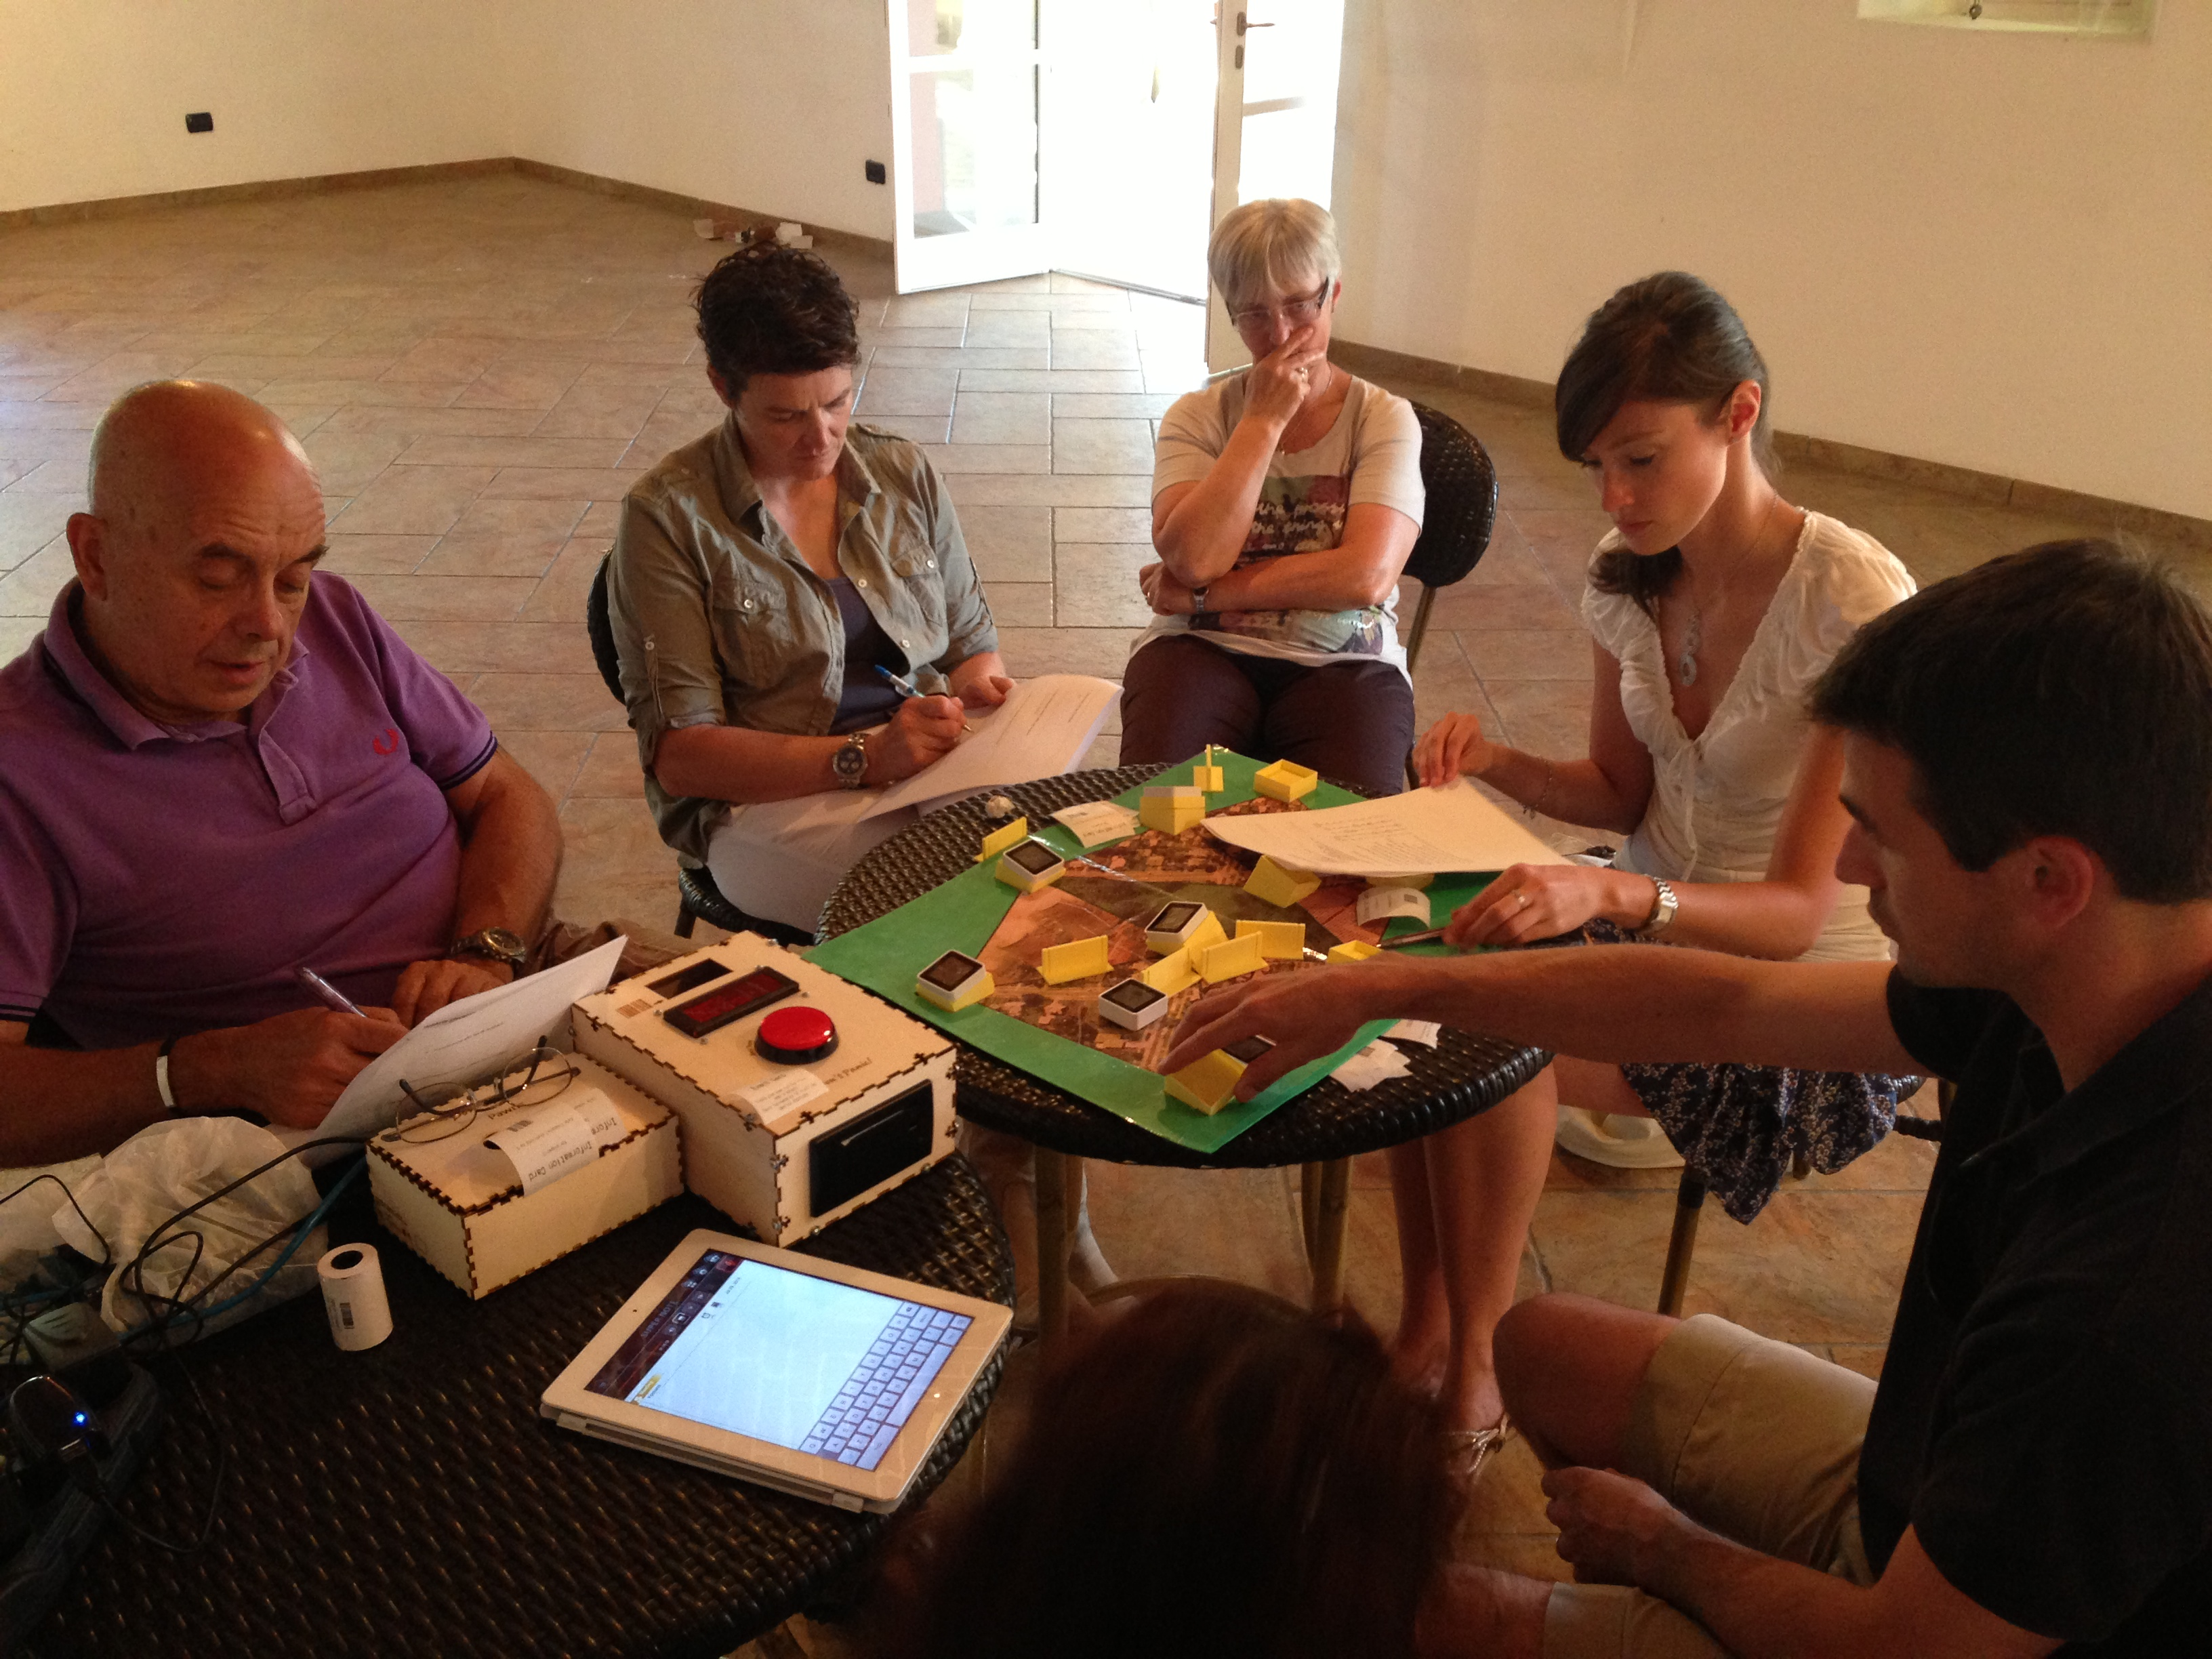
\includegraphics{imgs/d2_prototype.jpg}
\caption{Participants of the G3 group filling in SUS questionnaires,
after the test of D2 prototype}
\end{figure}

During focus groups low and high fidelity prototypes were evaluated.
Low-fidelity prototypes acted as technology probes
{[}@Hutchinson:2003il{]}. The typical setting of focus groups performed
is represented in Figure X. Despite their evident usability issues, they
were essential to create new scenarios of use and identify technological
and usage challenges. High-fidelity prototypes were usability tested
{[}@Dumas:2009th{]}, using a SUS scale {[}@jordan1996usability
pag.189{]}.

\subsubsection{The rigor cycle}\label{the-rigor-cycle}

The design work was grounded in literature about computer supported
reflective learning (Chapter X) and in sensing-based interaction
(Chapter Y). While the former identified \emph{what} activities and
processes to trigger reflection can be enhanced with technology; the
latter provided guidelines on \emph{how} to design user interfaces for
the technologies created.

Yet, as pointed out by Edelson {[}-@Edelson:2002kp{]}, ``design plays a
critical role in the development of theories, not just their
evaluation''. The work in this thesis contributed with knowledge useful
for validating the CSRL model described in {[}@Krogstie:fo{]} (as in
P2), in defining new theories about how technology can support
reflective learning (P6) and in drafting design challenges to develop
data capturing tools (P3).

Those constructs came as output of an effort towards generalising the
experience earned with the design and construction of prototypes, and
knowledge that surfaced from field studies to other application domains.
Research results were hence brought to domains that might benefit from
the novel interaction techniques to support reflection developed in this
research work. To accomplish this goal, I compared research results with
other case studies in the MIRROR project and I conducted research
abroad, as guest researcher, at City London University and MIT. During a
total of twenty-six weeks time abroad, I joined projects run by the
respective institutions doing design and prototypes construction work
inspired by the results of this PhD (Figure X).

\begin{figure}[htbp]
\centering
\includegraphics{imgs/london+mit.pdf}
\caption{Prototypes developed during research visit abroad}
\end{figure}

During fourteen weeks spent at City University (one of the partners of
the MIRROR consortium) I investigated the design and production of a
digitally augmented serious game for better training of dementia carers,
under the supervision of professor Neil Maiden. The game has been
implemented and evaluated in eight care homes in the greater London
area, and is reported in a joined publication to be submitted.

During twelve weeks spent at the MIT SENSEable City Lab I investigated
the design and production of a tangible interface to promote user
engagement and reflection about urban-mobility data under the
supervision of professor Carlo Ratti. The work has been has been
displayed to the public in two exhibitions: ``Wave'' currently held in
Paris and ``CNR Internet Festival'' held in Pisa,
Italy.\todo{these two paragraphs report on results. should be moved to another chapter?}

\subsection{Exploitation of research
results}\label{exploitation-of-research-results}

During the late phase of the research, the innovativeness of the
research performed has been evaluated and basis for a future
commercialisation of results have been settled. To this end, I joined
forces with NTNU Technology Transfer AS, a business facilitator
affiliated with NTNU. I also cooperated with the NTNU School of
Entrepreneurship {[}\^{}es{]} evaluating the market potential for the
technology tools developed.

I co-authored five declaration of inventions. The documents, formalising
description and contributors for the inventions, poses the grounds for
considering patenting and commercialising research results.

In order to asses the market value for the inventions I ran technology
benchmarks reported in Appendix
X\todo{should I add benchmarks and DOFIs in appendix?}. Benchmark
results were useful for selecting specific technologies and tools to be
employed in the production of prototypes. I also met several
representatives from the interests, showing research outcomes and
demoing prototypes. I took part in a design challenge at the MIT Media
Lab.

In November 2014 one of the invention won 150.00NOK
(\textasciitilde{}22.000USD) from NTNU Discovery \footnote{NTNU
  Discovery - http://ntnudiscovery.no} fund to continue innovation work
after the completion the PhD.
